\documentclass{article}
\usepackage[utf8]{inputenc}

\title{Theory of Universe}
\author{mikethielvoldt }
\date{December 2020}

\usepackage{natbib}
\usepackage{graphicx}

\begin{document}

\maketitle

\section{Introduction}
There is a theory which states that if ever anyone discovers exactly what the Universe is for and why it is here, it will instantly disappear and be replaced by something even more bizarre and inexplicable.
There is another theory which states that this has already happened.



\begin{figure}[h!]
\centering
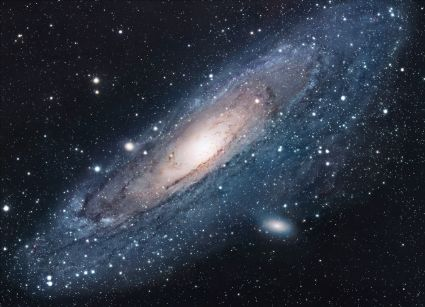
\includegraphics[scale=1.7]{galaxy}
\caption{galaxy}
\label{fig:galaxy}
\end{figure}

\section{Conclusion}
``I always thought something was fundamentally wrong with the universe'' \citep{adams1995hitchhiker}\newline
\newline
God does not play dice with the universe; He plays an ineffable game of His own devising, which might be compared, from the perspective of any of the other players [i.e. everybody], to being involved in an obscure and complex variant of poker in a pitch-dark room, with blank cards, for infinite stakes, with a Dealer who won't tell you the rules, and who \em{smiles all the time}.

\bibliographystyle{plain}
\bibliography{references}
\end{document}
